\newpage
\section{Revisão da Teoria}

\subsection{Modulação QPSK}

\begin{figure}[H]
  \centering
  \caption{Diagrama de blocos do modulador QPSK.}
  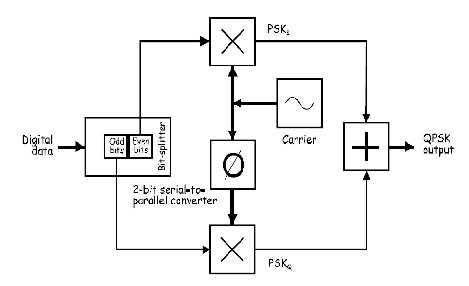
\includegraphics[scale=0.6]{tx}
  
  \small Fonte: iitg.vlab.co.in,. (2012). QPSK Modulation (Real time experiment).
  \label{fig:tx}
\end{figure}

Na entrada do modulador QPSK (figura \ref{fig:tx}), os bits de dados pares (isto é, bits 0, 2, 4, ..., etc) são removidos da sequência de dados através de um conversor serial-paralelo de 2 bits \cite{Couch} e são multiplicados com uma portadora para gerar um sinal BPSK (chamado de $PSK_I$, equalçao \ref{equ:PSKI}). 

\begin{equation}
  \label{equ:PSKI}
  PSK_I = A_c\cdot m_{par}(t) \cdot cos \left(2\pi f_c\right), \qquad m_{par}(t) = \, \mbox{1 ou -1.}
\end{equation}

Ao mesmo tempo, os bits impares (1, 3, 5, ..., etc), também são removidos da sequência de dados pelo conversor série-paralelo e alimentam um segundo modulador BPSK (chamado $PSK_Q$, equação \ref{equ:PSKQ}). 

\begin{equation}
  \label{equ:PSKQ}
  PSK_Q = A_c\cdot m_{impar}(t) \cdot sen \left(2\pi f_c\right), \qquad m_{impar}(t) = \, \mbox{1 ou -1.}
\end{equation}

Contudo, esse segundo modulador, PSKQ, possui uma defasagem de 90° em relação ao primeiro modulador, PSKI \cite{Carlson,Proakis}. Os dois sinais BPSK são, então, adicionados e transmitidos, com a mesma frequência de portadora, ou seja, são transmitidos dois sinais BPSK utilizando a mesma faixa de espectro. Isso é possível pois a diferênça de 90° entre a portadora do PSKI e do PSKQ permite que o receptor separe os dados usando discriminação por fase \cite{Lathi}. A figura \ref{fig:onda} mostra a forma de onda produzida pelo modulador QPSK.

\begin{figure}[H]
  \centering
  \caption{Forma de onda de saída do modulador QPSK.}
  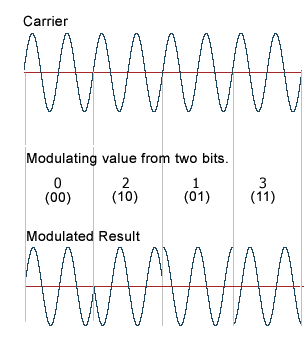
\includegraphics[scale=0.6]{onda}
  
  \small Fonte: iitg.vlab.co.in,. (2012). QPSK Modulation (Real time experiment).
  \label{fig:onda}
\end{figure}


O sinal resultante da modulação QPSK é descrito na equação \ref{equ:QPSK} \cite{Stallings}.

\begin{equation}
  \label{equ:QPSK}
  QPSK = A_c\cdot m_{par}(t) \cdot cos \left(2\pi f_c\right) + A_c\cdot m_{impar}(t) \cdot sen \left(2\pi f_c\right), \qquad m(t) = \, \mbox{1 ou -1.}
\end{equation}

A constelação do sinal QPSK é mostrada na figura \ref{fig:constelation}

\begin{figure}[H]
  \centering
  \caption{Constelação do sinal QPSK.}
  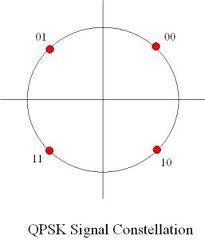
\includegraphics[scale=0.8]{constelation}
  
  \small Fonte: iitg.vlab.co.in,. (2012). QPSK Modulation (Real time experiment).
  \label{fig:constelation}
\end{figure}
                  

\subsection{Demodulação QPSK}

Para a demodulação do sinal QPSK, são utilizados dois detectores de produto simultaneamente \cite{Medeiros}. Os dois sinais de dados são então extraídos do sinal QPSK ao mesmo tempo. Os bits são identificados com o emprego de um integrador e um decisor. Em seguida, a mensagem é reconstruída utilizando um decisor, o qual define quais bits foram recebidos, e é recolocada na forma serial por um conversor paralelo-serial de 2 bits.

A figura \ref{fig:rx} mostra o diagrama de blocos para um demodulador QPSK. Note que, apesar dos detectores de produto utilizarem a mesma portadora de referência, em um deles a portadora está defasada de 90°.

\begin{figure}[H]
  \centering
  \caption{Diagrama de blocos do receptor QPSK.}
  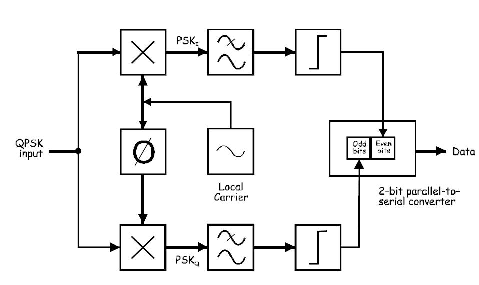
\includegraphics[scale=0.6]{rx}
  
  \small Fonte: iitg.vlab.co.in,. (2012). QPSK Modulation (Real time experiment).
  \label{fig:rx}
\end{figure}

